\documentclass[1p]{elsarticle_modified}
%\bibliographystyle{elsarticle-num}

%\usepackage[colorlinks]{hyperref}
%\usepackage{abbrmath_seonhwa} %\Abb, \Ascr, \Acal ,\Abf, \Afrak
\usepackage{amsfonts}
\usepackage{amssymb}
\usepackage{amsmath}
\usepackage{amsthm}
\usepackage{scalefnt}
\usepackage{amsbsy}
\usepackage{kotex}
\usepackage{caption}
\usepackage{subfig}
\usepackage{color}
\usepackage{graphicx}
\usepackage{xcolor} %% white, black, red, green, blue, cyan, magenta, yellow
\usepackage{float}
\usepackage{setspace}
\usepackage{hyperref}

\usepackage{tikz}
\usetikzlibrary{arrows}

\usepackage{multirow}
\usepackage{array} % fixed length table
\usepackage{hhline}

%%%%%%%%%%%%%%%%%%%%%
\makeatletter
\renewcommand*\env@matrix[1][\arraystretch]{%
	\edef\arraystretch{#1}%
	\hskip -\arraycolsep
	\let\@ifnextchar\new@ifnextchar
	\array{*\c@MaxMatrixCols c}}
\makeatother %https://tex.stackexchange.com/questions/14071/how-can-i-increase-the-line-spacing-in-a-matrix
%%%%%%%%%%%%%%%

\usepackage[normalem]{ulem}

\newcommand{\msout}[1]{\ifmmode\text{\sout{\ensuremath{#1}}}\else\sout{#1}\fi}
%SOURCE: \msout is \stkout macro in https://tex.stackexchange.com/questions/20609/strikeout-in-math-mode

\newcommand{\cancel}[1]{
	\ifmmode
	{\color{red}\msout{#1}}
	\else
	{\color{red}\sout{#1}}
	\fi
}

\newcommand{\add}[1]{
	{\color{blue}\uwave{#1}}
}

\newcommand{\replace}[2]{
	\ifmmode
	{\color{red}\msout{#1}}{\color{blue}\uwave{#2}}
	\else
	{\color{red}\sout{#1}}{\color{blue}\uwave{#2}}
	\fi
}

\newcommand{\Sol}{\mathcal{S}} %segment
\newcommand{\D}{D} %diagram
\newcommand{\A}{\mathcal{A}} %arc


%%%%%%%%%%%%%%%%%%%%%%%%%%%%%5 test

\def\sl{\operatorname{\textup{SL}}(2,\Cbb)}
\def\psl{\operatorname{\textup{PSL}}(2,\Cbb)}
\def\quan{\mkern 1mu \triangleright \mkern 1mu}

\theoremstyle{definition}
\newtheorem{thm}{Theorem}[section]
\newtheorem{prop}[thm]{Proposition}
\newtheorem{lem}[thm]{Lemma}
\newtheorem{ques}[thm]{Question}
\newtheorem{cor}[thm]{Corollary}
\newtheorem{defn}[thm]{Definition}
\newtheorem{exam}[thm]{Example}
\newtheorem{rmk}[thm]{Remark}
\newtheorem{alg}[thm]{Algorithm}

\newcommand{\I}{\sqrt{-1}}
\begin{document}

%\begin{frontmatter}
%
%\title{Boundary parabolic representations of knots up to 8 crossings}
%
%%% Group authors per affiliation:
%\author{Yunhi Cho} 
%\address{Department of Mathematics, University of Seoul, Seoul, Korea}
%\ead{yhcho@uos.ac.kr}
%
%
%\author{Seonhwa Kim} %\fnref{s_kim}}
%\address{Center for Geometry and Physics, Institute for Basic Science, Pohang, 37673, Korea}
%\ead{ryeona17@ibs.re.kr}
%
%\author{Hyuk Kim}
%\address{Department of Mathematical Sciences, Seoul National University, Seoul 08826, Korea}
%\ead{hyukkim@snu.ac.kr}
%
%\author{Seokbeom Yoon}
%\address{Department of Mathematical Sciences, Seoul National University, Seoul, 08826,  Korea}
%\ead{sbyoon15@snu.ac.kr}
%
%\begin{abstract}
%We find all boundary parabolic representation of knots up to 8 crossings.
%
%\end{abstract}
%\begin{keyword}
%    \MSC[2010] 57M25 
%\end{keyword}
%
%\end{frontmatter}

%\linenumbers
%\tableofcontents
%
\newcommand\colored[1]{\textcolor{white}{\rule[-0.35ex]{0.8em}{1.4ex}}\kern-0.8em\color{red} #1}%
%\newcommand\colored[1]{\textcolor{white}{ #1}\kern-2.17ex	\textcolor{white}{ #1}\kern-1.81ex	\textcolor{white}{ #1}\kern-2.15ex\color{red}#1	}

{\Large $\underline{12a_{0850}~(K12a_{0850})}$}

\setlength{\tabcolsep}{10pt}
\renewcommand{\arraystretch}{1.6}
\vspace{1cm}\begin{tabular}{m{100pt}>{\centering\arraybackslash}m{274pt}}
\multirow{5}{120pt}{
	\centering
	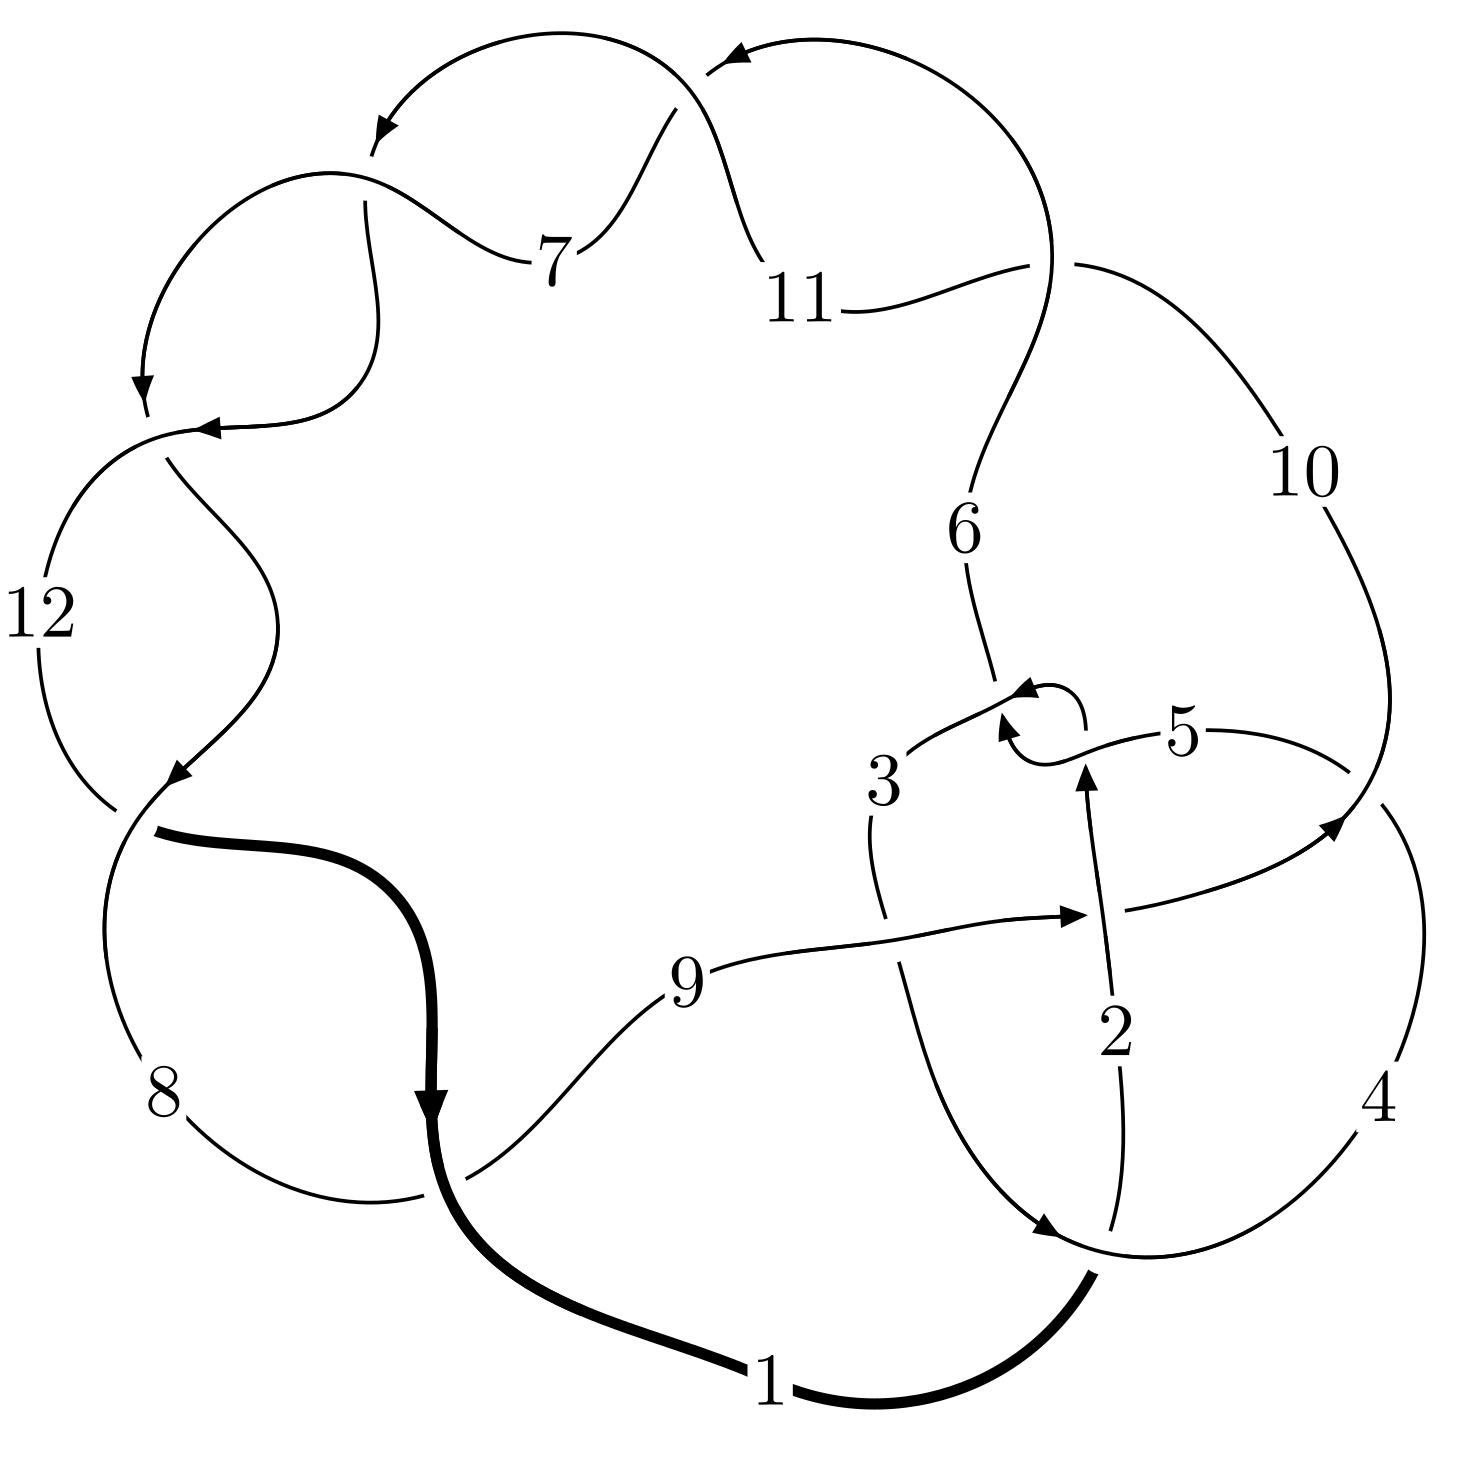
\includegraphics[width=112pt]{../../../GIT/diagram.site/Diagrams/png/1651_12a_0850.png}\\
\ \ \ A knot diagram\footnotemark}&
\allowdisplaybreaks
\textbf{Linearized knot diagam} \\
\cline{2-2}
 &
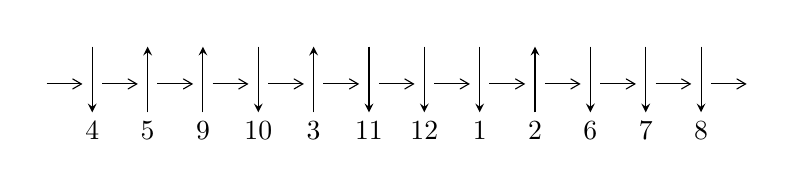
\begin{tikzpicture}[x=20pt, y=17pt]
	% nodes
	\node (C0) at (0, 0) {};
	\node (C1) at (1, 0) {};
	\node (C1U) at (1, +1) {};
	\node (C1D) at (1, -1) {4};

	\node (C2) at (2, 0) {};
	\node (C2U) at (2, +1) {};
	\node (C2D) at (2, -1) {5};

	\node (C3) at (3, 0) {};
	\node (C3U) at (3, +1) {};
	\node (C3D) at (3, -1) {9};

	\node (C4) at (4, 0) {};
	\node (C4U) at (4, +1) {};
	\node (C4D) at (4, -1) {10};

	\node (C5) at (5, 0) {};
	\node (C5U) at (5, +1) {};
	\node (C5D) at (5, -1) {3};

	\node (C6) at (6, 0) {};
	\node (C6U) at (6, +1) {};
	\node (C6D) at (6, -1) {11};

	\node (C7) at (7, 0) {};
	\node (C7U) at (7, +1) {};
	\node (C7D) at (7, -1) {12};

	\node (C8) at (8, 0) {};
	\node (C8U) at (8, +1) {};
	\node (C8D) at (8, -1) {1};

	\node (C9) at (9, 0) {};
	\node (C9U) at (9, +1) {};
	\node (C9D) at (9, -1) {2};

	\node (C10) at (10, 0) {};
	\node (C10U) at (10, +1) {};
	\node (C10D) at (10, -1) {6};

	\node (C11) at (11, 0) {};
	\node (C11U) at (11, +1) {};
	\node (C11D) at (11, -1) {7};

	\node (C12) at (12, 0) {};
	\node (C12U) at (12, +1) {};
	\node (C12D) at (12, -1) {8};
	\node (C13) at (13, 0) {};

	% arrows
	\draw[->,>={angle 60}]
	(C0) edge (C1) (C1) edge (C2) (C2) edge (C3) (C3) edge (C4) (C4) edge (C5) (C5) edge (C6) (C6) edge (C7) (C7) edge (C8) (C8) edge (C9) (C9) edge (C10) (C10) edge (C11) (C11) edge (C12) (C12) edge (C13) ;	\draw[->,>=stealth]
	(C1U) edge (C1D) (C2D) edge (C2U) (C3D) edge (C3U) (C4U) edge (C4D) (C5D) edge (C5U) (C6U) edge (C6D) (C7U) edge (C7D) (C8U) edge (C8D) (C9D) edge (C9U) (C10U) edge (C10D) (C11U) edge (C11D) (C12U) edge (C12D) ;
	\end{tikzpicture} \\
\hhline{~~} \\& 
\textbf{Solving Sequence} \\ \cline{2-2} 
 &
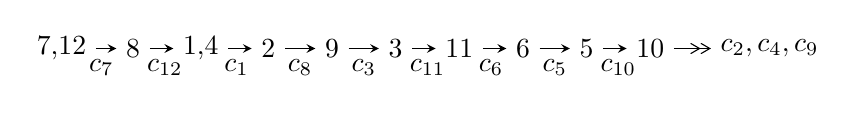
\begin{tikzpicture}[x=23pt, y=7pt]
	% node
	\node (A0) at (-1/8, 0) {7,12};
	\node (A1) at (1, 0) {8};
	\node (A2) at (33/16, 0) {1,4};
	\node (A3) at (25/8, 0) {2};
	\node (A4) at (33/8, 0) {9};
	\node (A5) at (41/8, 0) {3};
	\node (A6) at (49/8, 0) {11};
	\node (A7) at (57/8, 0) {6};
	\node (A8) at (65/8, 0) {5};
	\node (A9) at (73/8, 0) {10};
	\node (C1) at (1/2, -1) {$c_{7}$};
	\node (C2) at (3/2, -1) {$c_{12}$};
	\node (C3) at (21/8, -1) {$c_{1}$};
	\node (C4) at (29/8, -1) {$c_{8}$};
	\node (C5) at (37/8, -1) {$c_{3}$};
	\node (C6) at (45/8, -1) {$c_{11}$};
	\node (C7) at (53/8, -1) {$c_{6}$};
	\node (C8) at (61/8, -1) {$c_{5}$};
	\node (C9) at (69/8, -1) {$c_{10}$};
	\node (A10) at (11, 0) {$c_{2},c_{4},c_{9}$};

	% edge
	\draw[->,>=stealth]	
	(A0) edge (A1) (A1) edge (A2) (A2) edge (A3) (A3) edge (A4) (A4) edge (A5) (A5) edge (A6) (A6) edge (A7) (A7) edge (A8) (A8) edge (A9) ;
	\draw[->>,>={angle 60}]	
	(A9) edge (A10);
\end{tikzpicture} \\ 

\end{tabular} \\

\footnotetext{
The image of knot diagram is generated by the software ``\textbf{Draw programme}" developed by Andrew Bartholomew(\url{http://www.layer8.co.uk/maths/draw/index.htm\#Running-draw}), where we modified some parts for our purpose(\url{https://github.com/CATsTAILs/LinksPainter}).
}\phantom \\ \newline 
\centering \textbf{Ideals for irreducible components\footnotemark of $X_{\text{par}}$} 
 
\begin{align*}
I^u_{1}&=\langle 
-412178201122641 u^{45}-775553559035752 u^{44}+\cdots+353733604752049 b+614435998813861,\\
\phantom{I^u_{1}}&\phantom{= \langle  }402182189901230 u^{45}+1007252468993735 u^{44}+\cdots+353733604752049 a-1539279368053536,\\
\phantom{I^u_{1}}&\phantom{= \langle  }u^{46}+2 u^{45}+\cdots+u+1\rangle \\
I^u_{2}&=\langle 
b+1,\;a- u-1,\;u^2+u-1\rangle \\
\\
\end{align*}
\raggedright * 2 irreducible components of $\dim_{\mathbb{C}}=0$, with total 48 representations.\\
\footnotetext{All coefficients of polynomials are rational numbers. But the coefficients are sometimes approximated in decimal forms when there is not enough margin.}
\newpage
\renewcommand{\arraystretch}{1}
\centering \section*{I. $I^u_{1}= \langle -4.12\times10^{14} u^{45}-7.76\times10^{14} u^{44}+\cdots+3.54\times10^{14} b+6.14\times10^{14},\;4.02\times10^{14} u^{45}+1.01\times10^{15} u^{44}+\cdots+3.54\times10^{14} a-1.54\times10^{15},\;u^{46}+2 u^{45}+\cdots+u+1 \rangle$}
\flushleft \textbf{(i) Arc colorings}\\
\begin{tabular}{m{7pt} m{180pt} m{7pt} m{180pt} }
\flushright $a_{7}=$&$\begin{pmatrix}1\\0\end{pmatrix}$ \\
\flushright $a_{12}=$&$\begin{pmatrix}0\\u\end{pmatrix}$ \\
\flushright $a_{8}=$&$\begin{pmatrix}1\\u^2\end{pmatrix}$ \\
\flushright $a_{1}=$&$\begin{pmatrix}- u\\- u^3+u\end{pmatrix}$ \\
\flushright $a_{4}=$&$\begin{pmatrix}-1.13696 u^{45}-2.84749 u^{44}+\cdots+10.2682 u+4.35152\\1.16522 u^{45}+2.19248 u^{44}+\cdots-8.68849 u-1.73700\end{pmatrix}$ \\
\flushright $a_{2}=$&$\begin{pmatrix}1.82251 u^{45}+1.39735 u^{44}+\cdots-4.08553 u+0.311253\\2.24768 u^{45}-0.402662 u^{44}+\cdots+1.51126 u+1.82251\end{pmatrix}$ \\
\flushright $a_{9}=$&$\begin{pmatrix}- u^2+1\\- u^4+2 u^2\end{pmatrix}$ \\
\flushright $a_{3}=$&$\begin{pmatrix}-2.46826 u^{45}-5.24035 u^{44}+\cdots+19.2748 u+6.20584\\-0.0909725 u^{45}+1.39965 u^{44}+\cdots-6.03410 u-1.46820\end{pmatrix}$ \\
\flushright $a_{11}=$&$\begin{pmatrix}u\\u\end{pmatrix}$ \\
\flushright $a_{6}=$&$\begin{pmatrix}- u^2+1\\- u^2\end{pmatrix}$ \\
\flushright $a_{5}=$&$\begin{pmatrix}-1.96200 u^{45}-4.63888 u^{44}+\cdots+17.5120 u+6.75902\\0.311421 u^{45}+1.20112 u^{44}+\cdots-5.48102 u-0.962037\end{pmatrix}$ \\
\flushright $a_{10}=$&$\begin{pmatrix}- u^3+2 u\\- u^3+u\end{pmatrix}$\\&\end{tabular}
\flushleft \textbf{(ii) Obstruction class $= -1$}\\~\\
\flushleft \textbf{(iii) Cusp Shapes $= -\frac{473682658173898}{353733604752049} u^{45}-\frac{99045102071581}{353733604752049} u^{44}+\cdots+\frac{10709047957584936}{353733604752049} u+\frac{2653235649051613}{353733604752049}$}\\~\\
\newpage\renewcommand{\arraystretch}{1}
\flushleft \textbf{(iv) u-Polynomials at the component}\newline \\
\begin{tabular}{m{50pt}|m{274pt}}
Crossings & \hspace{64pt}u-Polynomials at each crossing \\
\hline $$\begin{aligned}c_{1}\end{aligned}$$&$\begin{aligned}
&u^{46}-7 u^{45}+\cdots-28 u+4
\end{aligned}$\\
\hline $$\begin{aligned}c_{2},c_{5}\end{aligned}$$&$\begin{aligned}
&u^{46}+3 u^{45}+\cdots+32 u+1
\end{aligned}$\\
\hline $$\begin{aligned}c_{3}\end{aligned}$$&$\begin{aligned}
&u^{46}+23 u^{44}+\cdots-59 u-1
\end{aligned}$\\
\hline $$\begin{aligned}c_{4}\end{aligned}$$&$\begin{aligned}
&u^{46}+2 u^{45}+\cdots-21 u-1
\end{aligned}$\\
\hline $$\begin{aligned}c_{6},c_{7},c_{8}\\c_{10},c_{11},c_{12}\end{aligned}$$&$\begin{aligned}
&u^{46}-2 u^{45}+\cdots- u+1
\end{aligned}$\\
\hline $$\begin{aligned}c_{9}\end{aligned}$$&$\begin{aligned}
&u^{46}+2 u^{45}+\cdots+u+1
\end{aligned}$\\
\hline
\end{tabular}\\~\\
\newpage\renewcommand{\arraystretch}{1}
\flushleft \textbf{(v) Riley Polynomials at the component}\newline \\
\begin{tabular}{m{50pt}|m{274pt}}
Crossings & \hspace{64pt}Riley Polynomials at each crossing \\
\hline $$\begin{aligned}c_{1}\end{aligned}$$&$\begin{aligned}
&y^{46}-15 y^{45}+\cdots-328 y+16
\end{aligned}$\\
\hline $$\begin{aligned}c_{2},c_{5}\end{aligned}$$&$\begin{aligned}
&y^{46}-25 y^{45}+\cdots-588 y+1
\end{aligned}$\\
\hline $$\begin{aligned}c_{3}\end{aligned}$$&$\begin{aligned}
&y^{46}+46 y^{45}+\cdots-3437 y+1
\end{aligned}$\\
\hline $$\begin{aligned}c_{4}\end{aligned}$$&$\begin{aligned}
&y^{46}+30 y^{45}+\cdots-445 y+1
\end{aligned}$\\
\hline $$\begin{aligned}c_{6},c_{7},c_{8}\\c_{10},c_{11},c_{12}\end{aligned}$$&$\begin{aligned}
&y^{46}-66 y^{45}+\cdots-9 y+1
\end{aligned}$\\
\hline $$\begin{aligned}c_{9}\end{aligned}$$&$\begin{aligned}
&y^{46}-10 y^{45}+\cdots-9 y+1
\end{aligned}$\\
\hline
\end{tabular}\\~\\
\newpage\flushleft \textbf{(vi) Complex Volumes and Cusp Shapes}
$$\begin{array}{c|c|c}  
\text{Solutions to }I^u_{1}& \I (\text{vol} + \sqrt{-1}CS) & \text{Cusp shape}\\
 \hline 
\begin{aligned}
u &= \phantom{-}0.767158 + 0.433545 I \\
a &= -0.152356 + 0.237919 I \\
b &= -0.608935 + 0.607878 I\end{aligned}
 & -0.20687 + 1.83894 I & -8.26616 - 3.43927 I \\ \hline\begin{aligned}
u &= \phantom{-}0.767158 - 0.433545 I \\
a &= -0.152356 - 0.237919 I \\
b &= -0.608935 - 0.607878 I\end{aligned}
 & -0.20687 - 1.83894 I & -8.26616 + 3.43927 I \\ \hline\begin{aligned}
u &= \phantom{-}1.14595\phantom{ +0.000000I} \\
a &= \phantom{-}1.66543\phantom{ +0.000000I} \\
b &= -0.824680\phantom{ +0.000000I}\end{aligned}
 & -1.55865\phantom{ +0.000000I} & \phantom{-0.000000 } 0 \\ \hline\begin{aligned}
u &= \phantom{-}1.191040 + 0.091569 I \\
a &= \phantom{-}0.269705 - 0.115985 I \\
b &= -0.231211 + 1.314110 I\end{aligned}
 & -3.16460 - 3.49316 I & \phantom{-0.000000 } 0 \\ \hline\begin{aligned}
u &= \phantom{-}1.191040 - 0.091569 I \\
a &= \phantom{-}0.269705 + 0.115985 I \\
b &= -0.231211 - 1.314110 I\end{aligned}
 & -3.16460 + 3.49316 I & \phantom{-0.000000 } 0 \\ \hline\begin{aligned}
u &= -1.224310 + 0.038292 I \\
a &= \phantom{-}0.57689 - 2.38554 I \\
b &= -0.16096 - 1.67792 I\end{aligned}
 & -4.65165 + 0.65229 I & \phantom{-0.000000 } 0 \\ \hline\begin{aligned}
u &= -1.224310 - 0.038292 I \\
a &= \phantom{-}0.57689 + 2.38554 I \\
b &= -0.16096 + 1.67792 I\end{aligned}
 & -4.65165 - 0.65229 I & \phantom{-0.000000 } 0 \\ \hline\begin{aligned}
u &= -0.594658 + 0.493055 I \\
a &= \phantom{-}0.569482 + 0.019769 I \\
b &= \phantom{-}1.216190 - 0.260596 I\end{aligned}
 & \phantom{-}0.76638 + 8.84991 I & -5.93176 - 9.09785 I \\ \hline\begin{aligned}
u &= -0.594658 - 0.493055 I \\
a &= \phantom{-}0.569482 - 0.019769 I \\
b &= \phantom{-}1.216190 + 0.260596 I\end{aligned}
 & \phantom{-}0.76638 - 8.84991 I & -5.93176 + 9.09785 I \\ \hline\begin{aligned}
u &= -1.223150 + 0.246640 I \\
a &= \phantom{-}0.481344 + 0.605666 I \\
b &= -0.206918 + 0.060427 I\end{aligned}
 & -6.68187 + 3.83644 I & \phantom{-0.000000 } 0\\
 \hline 
 \end{array}$$\newpage$$\begin{array}{c|c|c}  
\text{Solutions to }I^u_{1}& \I (\text{vol} + \sqrt{-1}CS) & \text{Cusp shape}\\
 \hline 
\begin{aligned}
u &= -1.223150 - 0.246640 I \\
a &= \phantom{-}0.481344 - 0.605666 I \\
b &= -0.206918 - 0.060427 I\end{aligned}
 & -6.68187 - 3.83644 I & \phantom{-0.000000 } 0 \\ \hline\begin{aligned}
u &= \phantom{-}1.280350 + 0.145473 I \\
a &= -1.341390 + 0.223322 I \\
b &= \phantom{-}0.232936 + 0.197353 I\end{aligned}
 & -8.55312 - 5.24786 I & \phantom{-0.000000 } 0 \\ \hline\begin{aligned}
u &= \phantom{-}1.280350 - 0.145473 I \\
a &= -1.341390 - 0.223322 I \\
b &= \phantom{-}0.232936 - 0.197353 I\end{aligned}
 & -8.55312 + 5.24786 I & \phantom{-0.000000 } 0 \\ \hline\begin{aligned}
u &= \phantom{-}1.280250 + 0.244696 I \\
a &= \phantom{-}1.346480 - 0.364424 I \\
b &= -0.045681 + 0.143330 I\end{aligned}
 & -5.29495 - 11.44320 I & \phantom{-0.000000 } 0 \\ \hline\begin{aligned}
u &= \phantom{-}1.280250 - 0.244696 I \\
a &= \phantom{-}1.346480 + 0.364424 I \\
b &= -0.045681 - 0.143330 I\end{aligned}
 & -5.29495 + 11.44320 I & \phantom{-0.000000 } 0 \\ \hline\begin{aligned}
u &= -0.605806 + 0.310686 I \\
a &= -0.880404 + 0.351414 I \\
b &= -1.112130 + 0.350962 I\end{aligned}
 & -2.39123 + 3.64692 I & -10.43839 - 7.63926 I \\ \hline\begin{aligned}
u &= -0.605806 - 0.310686 I \\
a &= -0.880404 - 0.351414 I \\
b &= -1.112130 - 0.350962 I\end{aligned}
 & -2.39123 - 3.64692 I & -10.43839 + 7.63926 I \\ \hline\begin{aligned}
u &= \phantom{-}0.454796 + 0.454478 I \\
a &= \phantom{-}0.539747 - 0.277523 I \\
b &= \phantom{-}0.450806 - 0.330065 I\end{aligned}
 & -1.27121 - 1.36834 I & -10.65988 + 5.78093 I \\ \hline\begin{aligned}
u &= \phantom{-}0.454796 - 0.454478 I \\
a &= \phantom{-}0.539747 + 0.277523 I \\
b &= \phantom{-}0.450806 + 0.330065 I\end{aligned}
 & -1.27121 + 1.36834 I & -10.65988 - 5.78093 I \\ \hline\begin{aligned}
u &= -1.377040 + 0.092167 I \\
a &= -0.832099 - 0.286390 I \\
b &= -0.267749 - 0.034492 I\end{aligned}
 & -7.56750 + 0.10369 I & \phantom{-0.000000 } 0\\
 \hline 
 \end{array}$$\newpage$$\begin{array}{c|c|c}  
\text{Solutions to }I^u_{1}& \I (\text{vol} + \sqrt{-1}CS) & \text{Cusp shape}\\
 \hline 
\begin{aligned}
u &= -1.377040 - 0.092167 I \\
a &= -0.832099 + 0.286390 I \\
b &= -0.267749 + 0.034492 I\end{aligned}
 & -7.56750 - 0.10369 I & \phantom{-0.000000 } 0 \\ \hline\begin{aligned}
u &= -0.073726 + 0.603893 I \\
a &= -0.64203 + 1.26805 I \\
b &= \phantom{-}0.0927429 - 0.0646432 I\end{aligned}
 & \phantom{-}2.34175 - 5.27392 I & -2.70147 + 5.21952 I \\ \hline\begin{aligned}
u &= -0.073726 - 0.603893 I \\
a &= -0.64203 - 1.26805 I \\
b &= \phantom{-}0.0927429 + 0.0646432 I\end{aligned}
 & \phantom{-}2.34175 + 5.27392 I & -2.70147 - 5.21952 I \\ \hline\begin{aligned}
u &= \phantom{-}0.550313\phantom{ +0.000000I} \\
a &= \phantom{-}0.180040\phantom{ +0.000000I} \\
b &= -0.495725\phantom{ +0.000000I}\end{aligned}
 & -0.914439\phantom{ +0.000000I} & -10.8210\phantom{ +0.000000I} \\ \hline\begin{aligned}
u &= -0.408387 + 0.270742 I \\
a &= -0.10890 + 2.30267 I \\
b &= \phantom{-}0.546367 + 0.446835 I\end{aligned}
 & \phantom{-}2.00550 + 2.33057 I & -1.71776 - 9.37052 I \\ \hline\begin{aligned}
u &= -0.408387 - 0.270742 I \\
a &= -0.10890 - 2.30267 I \\
b &= \phantom{-}0.546367 - 0.446835 I\end{aligned}
 & \phantom{-}2.00550 - 2.33057 I & -1.71776 + 9.37052 I \\ \hline\begin{aligned}
u &= -1.54354\phantom{ +0.000000I} \\
a &= -0.486260\phantom{ +0.000000I} \\
b &= -0.308213\phantom{ +0.000000I}\end{aligned}
 & -7.66046\phantom{ +0.000000I} & \phantom{-0.000000 } 0 \\ \hline\begin{aligned}
u &= \phantom{-}0.446300 + 0.095003 I \\
a &= \phantom{-}0.75867 - 2.98128 I \\
b &= -0.36758 + 1.78388 I\end{aligned}
 & \phantom{-}0.836196 - 0.200718 I & \phantom{-}20.7380 - 14.2709 I \\ \hline\begin{aligned}
u &= \phantom{-}0.446300 - 0.095003 I \\
a &= \phantom{-}0.75867 + 2.98128 I \\
b &= -0.36758 - 1.78388 I\end{aligned}
 & \phantom{-}0.836196 + 0.200718 I & \phantom{-}20.7380 + 14.2709 I \\ \hline\begin{aligned}
u &= \phantom{-}0.077400 + 0.391993 I \\
a &= \phantom{-}1.30428 - 0.97124 I \\
b &= \phantom{-}0.045336 - 0.233987 I\end{aligned}
 & -0.394888 - 1.327150 I & -5.21037 + 3.91369 I\\
 \hline 
 \end{array}$$\newpage$$\begin{array}{c|c|c}  
\text{Solutions to }I^u_{1}& \I (\text{vol} + \sqrt{-1}CS) & \text{Cusp shape}\\
 \hline 
\begin{aligned}
u &= \phantom{-}0.077400 - 0.391993 I \\
a &= \phantom{-}1.30428 + 0.97124 I \\
b &= \phantom{-}0.045336 + 0.233987 I\end{aligned}
 & -0.394888 + 1.327150 I & -5.21037 - 3.91369 I \\ \hline\begin{aligned}
u &= -0.186943 + 0.264216 I \\
a &= \phantom{-}1.76910 + 1.31460 I \\
b &= \phantom{-}1.040340 - 0.428302 I\end{aligned}
 & \phantom{-}2.61344 - 0.38254 I & \phantom{-}2.30820 - 3.85448 I \\ \hline\begin{aligned}
u &= -0.186943 - 0.264216 I \\
a &= \phantom{-}1.76910 - 1.31460 I \\
b &= \phantom{-}1.040340 + 0.428302 I\end{aligned}
 & \phantom{-}2.61344 + 0.38254 I & \phantom{-}2.30820 + 3.85448 I \\ \hline\begin{aligned}
u &= -1.77945\phantom{ +0.000000I} \\
a &= -3.67500\phantom{ +0.000000I} \\
b &= -6.90609\phantom{ +0.000000I}\end{aligned}
 & -12.3107\phantom{ +0.000000I} & \phantom{-0.000000 } 0 \\ \hline\begin{aligned}
u &= -1.78677 + 0.02018 I \\
a &= -0.70395 - 1.63402 I \\
b &= -1.35526 - 2.52294 I\end{aligned}
 & -14.1039 + 3.9673 I & \phantom{-0.000000 } 0 \\ \hline\begin{aligned}
u &= -1.78677 - 0.02018 I \\
a &= -0.70395 + 1.63402 I \\
b &= -1.35526 + 2.52294 I\end{aligned}
 & -14.1039 - 3.9673 I & \phantom{-0.000000 } 0 \\ \hline\begin{aligned}
u &= \phantom{-}1.79497 + 0.00903 I \\
a &= -1.32414 - 1.96060 I \\
b &= -2.65985 - 4.75153 I\end{aligned}
 & -15.7848 - 0.8615 I & \phantom{-0.000000 } 0 \\ \hline\begin{aligned}
u &= \phantom{-}1.79497 - 0.00903 I \\
a &= -1.32414 + 1.96060 I \\
b &= -2.65985 + 4.75153 I\end{aligned}
 & -15.7848 + 0.8615 I & \phantom{-0.000000 } 0 \\ \hline\begin{aligned}
u &= \phantom{-}1.79436 + 0.06450 I \\
a &= -1.58447 + 0.56774 I \\
b &= -3.05444 + 1.14510 I\end{aligned}
 & -17.7122 - 5.2449 I & \phantom{-0.000000 } 0 \\ \hline\begin{aligned}
u &= \phantom{-}1.79436 - 0.06450 I \\
a &= -1.58447 - 0.56774 I \\
b &= -3.05444 - 1.14510 I\end{aligned}
 & -17.7122 + 5.2449 I & \phantom{-0.000000 } 0\\
 \hline 
 \end{array}$$\newpage$$\begin{array}{c|c|c}  
\text{Solutions to }I^u_{1}& \I (\text{vol} + \sqrt{-1}CS) & \text{Cusp shape}\\
 \hline 
\begin{aligned}
u &= -1.80654 + 0.03660 I \\
a &= \phantom{-}2.93105 - 0.19688 I \\
b &= \phantom{-}5.72048 - 0.32024 I\end{aligned}
 & \phantom{-}19.5334 + 6.0912 I & \phantom{-0.000000 } 0 \\ \hline\begin{aligned}
u &= -1.80654 - 0.03660 I \\
a &= \phantom{-}2.93105 + 0.19688 I \\
b &= \phantom{-}5.72048 + 0.32024 I\end{aligned}
 & \phantom{-}19.5334 - 6.0912 I & \phantom{-0.000000 } 0 \\ \hline\begin{aligned}
u &= -1.80661 + 0.06306 I \\
a &= -2.75336 - 0.16817 I \\
b &= -5.50064 - 0.25278 I\end{aligned}
 & -16.6222 + 12.8685 I & \phantom{-0.000000 } 0 \\ \hline\begin{aligned}
u &= -1.80661 - 0.06306 I \\
a &= -2.75336 + 0.16817 I \\
b &= -5.50064 + 0.25278 I\end{aligned}
 & -16.6222 - 12.8685 I & \phantom{-0.000000 } 0 \\ \hline\begin{aligned}
u &= \phantom{-}1.82069 + 0.02719 I \\
a &= \phantom{-}1.93426 - 0.40849 I \\
b &= \phantom{-}3.99351 - 0.87975 I\end{aligned}
 & -19.3942 - 0.7197 I & \phantom{-0.000000 } 0 \\ \hline\begin{aligned}
u &= \phantom{-}1.82069 - 0.02719 I \\
a &= \phantom{-}1.93426 + 0.40849 I \\
b &= \phantom{-}3.99351 + 0.87975 I\end{aligned}
 & -19.3942 + 0.7197 I & \phantom{-0.000000 } 0\\
 \hline 
 \end{array}$$\newpage\newpage\renewcommand{\arraystretch}{1}
\centering \section*{II. $I^u_{2}= \langle b+1,\;a- u-1,\;u^2+u-1 \rangle$}
\flushleft \textbf{(i) Arc colorings}\\
\begin{tabular}{m{7pt} m{180pt} m{7pt} m{180pt} }
\flushright $a_{7}=$&$\begin{pmatrix}1\\0\end{pmatrix}$ \\
\flushright $a_{12}=$&$\begin{pmatrix}0\\u\end{pmatrix}$ \\
\flushright $a_{8}=$&$\begin{pmatrix}1\\- u+1\end{pmatrix}$ \\
\flushright $a_{1}=$&$\begin{pmatrix}- u\\- u+1\end{pmatrix}$ \\
\flushright $a_{4}=$&$\begin{pmatrix}u+1\\-1\end{pmatrix}$ \\
\flushright $a_{2}=$&$\begin{pmatrix}- u\\- u+1\end{pmatrix}$ \\
\flushright $a_{9}=$&$\begin{pmatrix}u\\u\end{pmatrix}$ \\
\flushright $a_{3}=$&$\begin{pmatrix}u+2\\0\end{pmatrix}$ \\
\flushright $a_{11}=$&$\begin{pmatrix}u\\u\end{pmatrix}$ \\
\flushright $a_{6}=$&$\begin{pmatrix}u\\u-1\end{pmatrix}$ \\
\flushright $a_{5}=$&$\begin{pmatrix}2 u+2\\u-1\end{pmatrix}$ \\
\flushright $a_{10}=$&$\begin{pmatrix}1\\- u+1\end{pmatrix}$\\&\end{tabular}
\flushleft \textbf{(ii) Obstruction class $= 1$}\\~\\
\flushleft \textbf{(iii) Cusp Shapes $= 1$}\\~\\
\newpage\renewcommand{\arraystretch}{1}
\flushleft \textbf{(iv) u-Polynomials at the component}\newline \\
\begin{tabular}{m{50pt}|m{274pt}}
Crossings & \hspace{64pt}u-Polynomials at each crossing \\
\hline $$\begin{aligned}c_{1}\end{aligned}$$&$\begin{aligned}
&u^2
\end{aligned}$\\
\hline $$\begin{aligned}c_{2}\end{aligned}$$&$\begin{aligned}
&(u+1)^2
\end{aligned}$\\
\hline $$\begin{aligned}c_{3},c_{4},c_{10}\\c_{11},c_{12}\end{aligned}$$&$\begin{aligned}
&u^2- u-1
\end{aligned}$\\
\hline $$\begin{aligned}c_{5}\end{aligned}$$&$\begin{aligned}
&(u-1)^2
\end{aligned}$\\
\hline $$\begin{aligned}c_{6},c_{7},c_{8}\\c_{9}\end{aligned}$$&$\begin{aligned}
&u^2+u-1
\end{aligned}$\\
\hline
\end{tabular}\\~\\
\newpage\renewcommand{\arraystretch}{1}
\flushleft \textbf{(v) Riley Polynomials at the component}\newline \\
\begin{tabular}{m{50pt}|m{274pt}}
Crossings & \hspace{64pt}Riley Polynomials at each crossing \\
\hline $$\begin{aligned}c_{1}\end{aligned}$$&$\begin{aligned}
&y^2
\end{aligned}$\\
\hline $$\begin{aligned}c_{2},c_{5}\end{aligned}$$&$\begin{aligned}
&(y-1)^2
\end{aligned}$\\
\hline $$\begin{aligned}c_{3},c_{4},c_{6}\\c_{7},c_{8},c_{9}\\c_{10},c_{11},c_{12}\end{aligned}$$&$\begin{aligned}
&y^2-3 y+1
\end{aligned}$\\
\hline
\end{tabular}\\~\\
\newpage\flushleft \textbf{(vi) Complex Volumes and Cusp Shapes}
$$\begin{array}{c|c|c}  
\text{Solutions to }I^u_{2}& \I (\text{vol} + \sqrt{-1}CS) & \text{Cusp shape}\\
 \hline 
\begin{aligned}
u &= \phantom{-}0.618034\phantom{ +0.000000I} \\
a &= \phantom{-}1.61803\phantom{ +0.000000I} \\
b &= -1.00000\phantom{ +0.000000I}\end{aligned}
 & \phantom{-}0.657974\phantom{ +0.000000I} & \phantom{-}1.00000\phantom{ +0.000000I} \\ \hline\begin{aligned}
u &= -1.61803\phantom{ +0.000000I} \\
a &= -0.618034\phantom{ +0.000000I} \\
b &= -1.00000\phantom{ +0.000000I}\end{aligned}
 & -7.23771\phantom{ +0.000000I} & \phantom{-}1.00000\phantom{ +0.000000I}\\
 \hline 
 \end{array}$$\newpage
\newpage\renewcommand{\arraystretch}{1}
\centering \section*{ III. u-Polynomials}
\begin{tabular}{m{50pt}|m{274pt}}
Crossings & \hspace{64pt}u-Polynomials at each crossing \\
\hline $$\begin{aligned}c_{1}\end{aligned}$$&$\begin{aligned}
&u^2(u^{46}-7 u^{45}+\cdots-28 u+4)
\end{aligned}$\\
\hline $$\begin{aligned}c_{2}\end{aligned}$$&$\begin{aligned}
&((u+1)^2)(u^{46}+3 u^{45}+\cdots+32 u+1)
\end{aligned}$\\
\hline $$\begin{aligned}c_{3}\end{aligned}$$&$\begin{aligned}
&(u^2- u-1)(u^{46}+23 u^{44}+\cdots-59 u-1)
\end{aligned}$\\
\hline $$\begin{aligned}c_{4}\end{aligned}$$&$\begin{aligned}
&(u^2- u-1)(u^{46}+2 u^{45}+\cdots-21 u-1)
\end{aligned}$\\
\hline $$\begin{aligned}c_{5}\end{aligned}$$&$\begin{aligned}
&((u-1)^2)(u^{46}+3 u^{45}+\cdots+32 u+1)
\end{aligned}$\\
\hline $$\begin{aligned}c_{6},c_{7},c_{8}\end{aligned}$$&$\begin{aligned}
&(u^2+u-1)(u^{46}-2 u^{45}+\cdots- u+1)
\end{aligned}$\\
\hline $$\begin{aligned}c_{9}\end{aligned}$$&$\begin{aligned}
&(u^2+u-1)(u^{46}+2 u^{45}+\cdots+u+1)
\end{aligned}$\\
\hline $$\begin{aligned}c_{10},c_{11},c_{12}\end{aligned}$$&$\begin{aligned}
&(u^2- u-1)(u^{46}-2 u^{45}+\cdots- u+1)
\end{aligned}$\\
\hline
\end{tabular}\newpage\renewcommand{\arraystretch}{1}
\centering \section*{ IV. Riley Polynomials}
\begin{tabular}{m{50pt}|m{274pt}}
Crossings & \hspace{64pt}Riley Polynomials at each crossing \\
\hline $$\begin{aligned}c_{1}\end{aligned}$$&$\begin{aligned}
&y^2(y^{46}-15 y^{45}+\cdots-328 y+16)
\end{aligned}$\\
\hline $$\begin{aligned}c_{2},c_{5}\end{aligned}$$&$\begin{aligned}
&((y-1)^2)(y^{46}-25 y^{45}+\cdots-588 y+1)
\end{aligned}$\\
\hline $$\begin{aligned}c_{3}\end{aligned}$$&$\begin{aligned}
&(y^2-3 y+1)(y^{46}+46 y^{45}+\cdots-3437 y+1)
\end{aligned}$\\
\hline $$\begin{aligned}c_{4}\end{aligned}$$&$\begin{aligned}
&(y^2-3 y+1)(y^{46}+30 y^{45}+\cdots-445 y+1)
\end{aligned}$\\
\hline $$\begin{aligned}c_{6},c_{7},c_{8}\\c_{10},c_{11},c_{12}\end{aligned}$$&$\begin{aligned}
&(y^2-3 y+1)(y^{46}-66 y^{45}+\cdots-9 y+1)
\end{aligned}$\\
\hline $$\begin{aligned}c_{9}\end{aligned}$$&$\begin{aligned}
&(y^2-3 y+1)(y^{46}-10 y^{45}+\cdots-9 y+1)
\end{aligned}$\\
\hline
\end{tabular}
\vskip 2pc
\end{document}